\documentclass[]{article}

%\usepackage{showframe} % To render a frame marking the margins 

\usepackage{tikz}
\usetikzlibrary{
    angles,
    arrows.meta,
    automata, % to use \node[state]
    graphs,
    intersections,
    quotes,
    positioning
}
\usepackage{amsmath, amssymb} % for $\therefore e_{l} * e_{r} \implies e_{r}$

% epigraph for quote at start of section
\usepackage{epigraph}
\setlength\epigraphwidth{8cm}
\setlength\epigraphrule{0pt}
\renewcommand{\epigraphsize}{\small\itshape}

% for hyperlinks and URL links
\usepackage{hyperref}

\title{\LaTeX{} Experiments\\ Part III: PGF/TikZ}

\author{AeAeA}

\begin{document}

\maketitle

\vspace{20pt}

\begin{figure}[h] \centering
    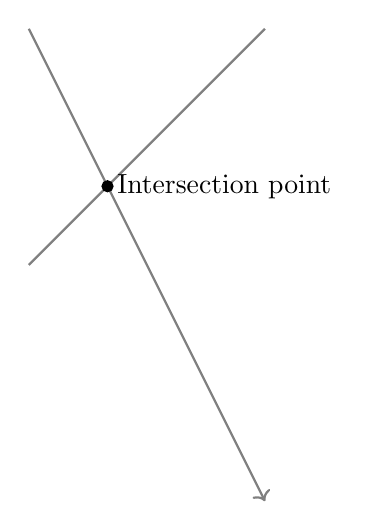
\begin{tikzpicture}
        \draw[gray, thick, ->] (-1,2) -- (2,-4);
        \draw[gray, thick] (-1,-1) -- (2,2);
        \filldraw[black] (0,0) circle (2pt) node[anchor=west] {Intersection point};
    \end{tikzpicture}
\end{figure}

%==============================================================================
\section{TikZ ist {\itshape kein} Zeichenprogramm}

\epigraph
{Für meinen Vater, damit er noch viele schöne TEX-Graphiken erschaffen kann.}
{--- \textup{Till Tantau}, PGF Manual}

\begin{itemize}
    \item \url{https://en.wikipedia.org/wiki/PGF/TikZ}
    \item \url{https://www.ctan.org/pkg/pgf}
    \item \url{https://github.com/pgf-tikz/pgf}
    \item \href{http://cremeronline.com/LaTeX/minimaltikz.pdf}
               {Minimal introduction to TikZ (unofficial)}
    \item  It comes with very good documentation; the version 3.1.5b of the 
           \href{http://mirrors.ctan.org/graphics/pgf/base/doc/pgfmanual.pdf}
                {PGF Manual} has over 1,300 pages (!) \ldots
    \item \ldots and an extensive collection of examples: \\
          \url{http://www.texample.net/tikz/}
    \item \url{https://en.wikibooks.org/wiki/LaTeX/PGF/TikZ}
    \item \url{https://www.overleaf.com/learn/latex/TikZ_package}
\end{itemize}



%--------------------------------------
\subsection{Basic elements: points, lines and paths}

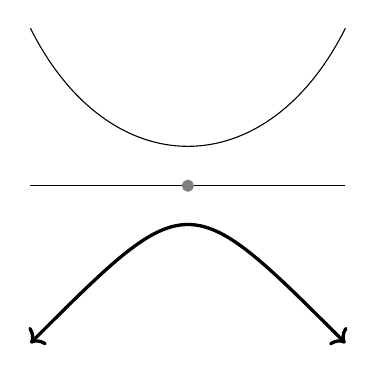
\begin{tikzpicture}
    \draw (-2,0) -- (2,0);
    \filldraw [gray] (0,0) circle (2pt);
    \draw[very thick, <->] (-2,-2) .. controls (0,0) .. (2,-2);
    \draw (-2,2) .. controls (-1,0) and (1,0) .. (2,2); 
\end{tikzpicture}

%--------------------------------------
\subsection{Basic geometric shapes: Circles, ellipses and polygons}

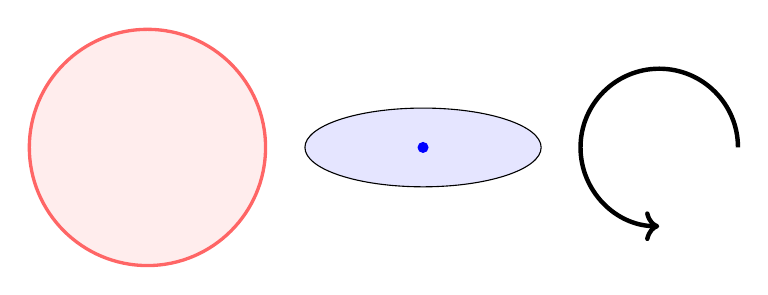
\begin{tikzpicture}
    \filldraw[color=red!60, fill=red!7, very thick] (-1,0) circle (1.5);
    \fill[blue!10] (2.5,0) ellipse (1.5 and 0.5);
    \fill[blue]    (2.5,0) circle (2pt);
    \draw (2.5,0) ellipse [x radius=1.5, y radius=0.5];
    \draw[ultra thick, ->] (6.5,0) arc (0:270:1);
\end{tikzpicture}

\vspace{20pt}

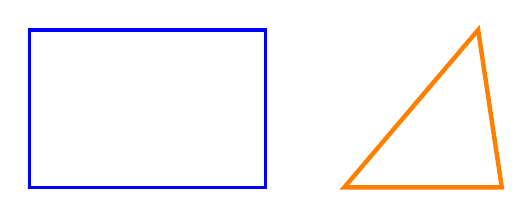
\begin{tikzpicture}
    \draw[blue, very thick] (0,0) rectangle (3,2);
    \draw[orange, ultra thick] (4,0) -- (6,0) -- (5.7,2) -- cycle;
\end{tikzpicture}

The code for the little "turned" ellipse 
\tikz \draw[rotate=30] (0,0) ellipse [x radius=6pt,y radius=3pt]; is \\
\verb+\tikz \draw[rotate=30] (0,0) ellipse [x radius=6pt,y radius=3pt];+

%--------------------------------------
\subsection{Elliptical arc}
%  \usetikzlibrary {arrows.meta}
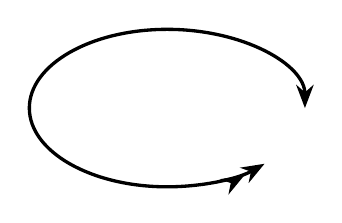
\begin{tikzpicture}[>=Stealth]
    \draw[<->>,very thick] 
        (0,0) arc [start angle=0, end angle=315, x radius=1.75cm, y radius=1cm];
\end{tikzpicture}

%--------------------------------------
\subsection{Arrow tips}

\marginpar{\texttt{Stealth}\\
\tikz [>=Stealth] \draw[<<<<-,ultra thick] (0,0) -- (0.1pt,0);}

\epigraph
{Karl wonders whether such a military name for the arrow type is really necessary. 
He is not really mollified when his son tells him that Microsoft’s PowerPoint 
uses the same name. He decides to have his students discuss this at some point.}
{--- \textup{Till Tantau}, PGF Manual}

This is an example of \texttt{Stealth} arrow tip 
\tikz [>=Stealth]
    \draw[<<-,ultra thick] (1,0) -- (1.5cm,10pt) -- (2cm,0pt) -- (2.5cm,10pt);
which is a “stealth-fighter-like”.

All arrow tips:\\
%  \usetikzlibrary {arrows.meta}
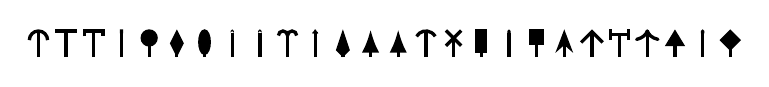
\begin{tikzpicture} [->,very thick]
    \draw[>=Arc Barb]      (0,0) -- (0,10pt);
    \draw[>=Bar]           (10pt,0) -- (10pt,10pt);
    \draw[>=Bracket]       (20pt,0) -- (20pt,10pt);
    \draw[>=Butt Cap]      (30pt,0) -- (30pt,10pt);
    \draw[>=Circle]        (40pt,0) -- (40pt,10pt);
    \draw[>=Diamond]       (50pt,0) -- (50pt,10pt);
    \draw[>=Ellipse]       (60pt,0) -- (60pt,10pt);
    \draw[>=Fast Round]    (70pt,0) -- (70pt,10pt);
    \draw[>=Fast Triangle] (80pt,0) -- (80pt,10pt);
    \draw[>=Hooks]         (90pt,0) -- (90pt,10pt);
    \draw[>=Implies]       (100pt,0) -- (100pt,10pt);
    \draw[>=Kite]          (110pt,0) -- (110pt,10pt);
    \draw[>=LaTeX]         (120pt,0) -- (120pt,10pt);
    \draw[>=Latex]         (130pt,0) -- (130pt,10pt);
    \draw[>=Parenthesis]   (140pt,0) -- (140pt,10pt);
    \draw[>=Rays]          (150pt,0) -- (150pt,10pt);
    \draw[>=Rectangle]     (160pt,0) -- (160pt,10pt);
    \draw[>=Round Cap]     (170pt,0) -- (170pt,10pt);
    \draw[>=Square]        (180pt,0) -- (180pt,10pt);
    \draw[>=Stealth]       (190pt,0) -- (190pt,10pt);
    \draw[>=Straight Barb] (200pt,0) -- (200pt,10pt);
    \draw[>=Tee Barb]      (210pt,0) -- (210pt,10pt);
    \draw[>=To]            (220pt,0) -- (220pt,10pt);
    \draw[>=Triangle]      (230pt,0) -- (230pt,10pt);
    \draw[>=Triangle Cap]  (240pt,0) -- (240pt,10pt);
    \draw[>=Turned Square] (250pt,0) -- (250pt,10pt);
\end{tikzpicture}

\marginpar{\tikz \draw[-To,red,ultra thick] (0,0) -- (0.1pt,0);}
(Almost) zero-length arrow: 
\tikz \draw[-To,red,ultra thick] (0,0) -- (0.1pt,0);

\subsubsection{Arrow Tip Kind \texttt{Implies}}
\marginpar{$\therefore\\ e_{l} * e_{r} \implies e_{r}$}
This arrow tip makes only sense in conjunction with the double option:
attach it to a double line to get something 
( \tikz \draw[double equal sign distance, -Implies] (0,0) -- (15pt,0); ) 
that looks like 
\texttt{amsmath} \TeX’s \verb+\implies+ arrow ( $\implies$ ). 
A typical use of this arrow tip is:\\
% \usetikzlibrary {arrows.meta,graphs}
\tikz \graph [
    clockwise=3, math nodes, edges = {double equal sign distance, -Implies}
] { 
    "\alpha", "\beta", "\gamma";
    "\alpha" -> "\beta" -> "\gamma" -> "\alpha"
};


%--------------------------------------
\subsection{Path}

\tikz \draw[thick,rounded corners=8pt]
    (0,0) -- (0,2) -- (1,3.25) -- (2,2) -- (2,0) -- (0,2) -- (2,2) -- (0,0) -- (2,0);

%--------------------------------------
\subsection{Curved path}

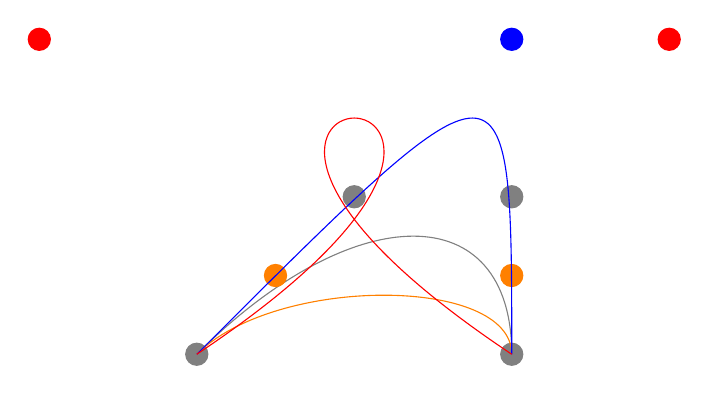
\begin{tikzpicture}[scale=2]
    \filldraw[gray] (0,0) circle [radius=2pt]
                    (1,1) circle [radius=2pt] 
                    (2,1) circle [radius=2pt] 
                    (2,0) circle [radius=2pt];
    \draw[gray] (0,0) .. controls (1,1) and (2,1) .. (2,0);

    \filldraw[orange] (0.5,0.5) circle [radius=2pt]
                      (2,0.5) circle [radius=2pt];                
    \draw[orange] (0,0) .. controls (0.5,0.5) and (2,0.5) .. (2,0);

    \filldraw[blue] (2,2) circle [radius=2pt];
    \draw[blue] (0,0) .. controls (2,2) .. (2,0);

    \filldraw[red] (3,2) circle [radius=2pt]
                   (-1,2) circle [radius=2pt];                
    \draw[red] (0,0) .. controls (3,2) and (-1,2) .. (2,0);
\end{tikzpicture}

%--------------------------------------
\subsection{Grid}
\marginpar{\tikz \draw[step=2pt] (0,0) grid (10pt,10pt);}
The code \verb+\tikz \draw[step=2pt] (0,0) grid (10pt,10pt);+ produces
\tikz \draw[step=2pt] (0,0) grid (10pt,10pt);.

Here is a bigger grid:\\
\tikz{ 
    \fill[orange] (0,0) circle (2pt);
    \fill[red] (50pt,50pt) circle (2pt);
    \fill[blue] (100pt,100pt) circle (2pt);

    \draw[step=5pt,gray,very thin] (1pt,1pt) grid (99pt,99pt);

    \draw (50pt,0) -- (50pt,100pt); % vertical
    \draw (0,50pt) -- (100pt,50pt); % horizontal
}

%--------------------------------------
\subsection{Circle and curved path}
\marginpar{0.555}
0.555 is the magic number.\\
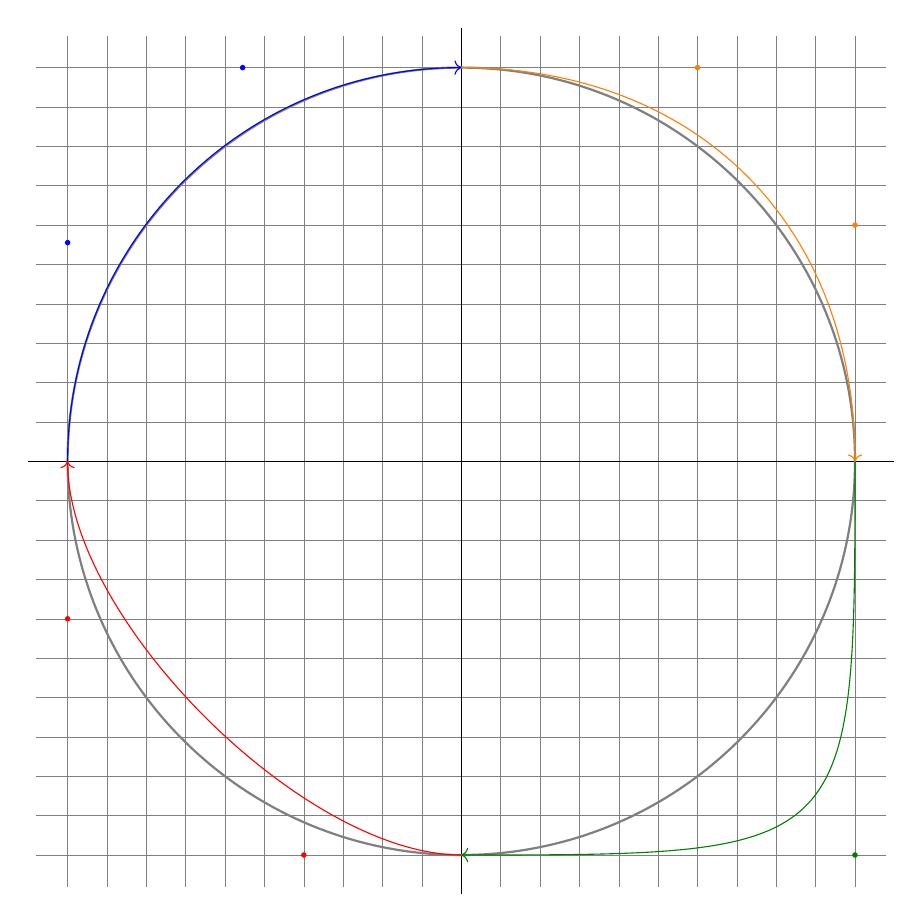
\begin{tikzpicture} [
    dark green/.style = {green!50!black}
]
    \draw[step=.5cm,gray,very thin] (-5.4,-5.4) grid (5.4,5.4); 

    \draw (-5.5,0) -- (5.5,0);
    \draw (0,-5.5) -- (0,5.5);

    \draw[gray,thick] (0,0) circle [radius=5cm];

    % 2.777 = 5 * 0.555(5)

    \fill[blue] (-5,2.777) circle (1pt) (-2.777,5) circle (1pt);
    \draw[blue,->] (-5,0) .. controls (-5,2.777) and (-2.777,5) .. (0,5);

    \fill[orange] (3,5) circle (1pt) (5,3) circle (1pt);
    \draw[orange,->] (0,5) .. controls (3,5) and (5,3) .. (5,0);

    \fill[dark green] (5,-5) circle (1pt);
    \draw[dark green,->] (5,0) .. controls (5,-5) .. (0,-5);

    \fill[red] (-2,-5) circle (1pt) (-5,-2) circle (1pt);
    \draw[red,->] (0,-5) .. controls (-2,-5) and (-5,-2) .. (-5,0);
\end{tikzpicture}

%--------------------------------------
\subsection{Clipping a path}
Original drawing on the left, clipped (and 1.4 scaled) drawing on the right:\\
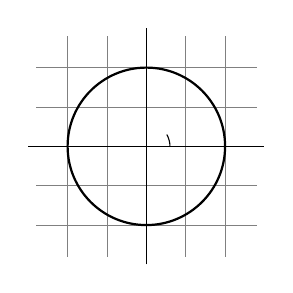
\begin{tikzpicture}
    \draw[step=.5cm,gray,very thin] (-1.4,-1.4) grid (1.4,1.4); 
    \draw (-1.5,0) -- (1.5,0);
    \draw (0,-1.5) -- (0,1.5);
    \draw[thick] (0,0) circle (1);
    \draw (0.3,0) arc [start angle=0, end angle=30, radius=0.3];
\end{tikzpicture}
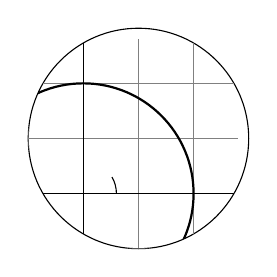
\begin{tikzpicture}[scale=1.4]
    \path[draw,clip] (0.5,0.5) circle (1);
    \draw[step=.5cm,gray,very thin] (-1.4,-1.4) grid (1.4,1.4); 
    \draw (-1.5,0) -- (1.5,0);
    \draw (0,-1.5) -- (0,1.5);
    \draw[thick] (0,0) circle (1);
    \draw (0.3,0) arc [start angle=0, end angle=30, radius=0.3];
\end{tikzpicture}

%--------------------------------------
\subsection{Parabola and Sine}
\marginpar{
    \tikz \draw[x=1.57ex,y=1ex] (0,0) sin (1,1) cos (2,0) sin (3,-1) cos (4,0) 
(0,1) cos (1,0) sin (2,-1) cos (3,0) sin (4,1);
}
Two parabolas 
\tikz \draw[x=2ex,y=2ex] (-1,0) rectangle (1,1) (-1,1) parabola (0,0) parabola (1,1);
and a parabola with placed bend 
\tikz \draw[x=2ex,y=2ex] (-1,0) rectangle (1,1) (-1,1) parabola bend (0,0) (1,1);

A parabola with the bend:
\tikz \draw[x=1pt,y=1pt] (0,0) parabola bend (4,16) (6,12);

A sine \tikz \draw[x=1ex,y=1ex] (0,0) sin (1.57,1); curve, 
and a longer span of sine and cosine: 
\tikz \draw[x=1.57ex,y=1ex] (0,0) sin (1,1) cos (2,0) sin (3,-1) cos (4,0) 
                            (0,1) cos (1,0) sin (2,-1) cos (3,0) sin (4,1);

%--------------------------------------
\subsection{Closing the path}
The \texttt{--cycle} causes the current path to be closed (actually the current part of 
the current path) by smoothly joining the first and last point. To appreciate 
the difference, consider the following example:\\
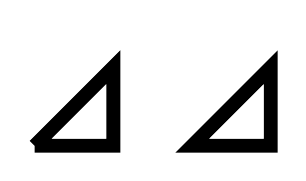
\begin{tikzpicture}[line width=5pt]
    \draw (0,0) -- (1,0) -- (1,1) -- (0,0);
    \draw (2,0) -- (3,0) -- (3,1) -- cycle; 
    \useasboundingbox (0,1.5); % make bounding box higher
\end{tikzpicture}

%--------------------------------------
\subsection{Shading}
\marginpar{\tikz \shade[ball color=green] (.5,.5) circle (.5);}
The default shading is a smooth transition from gray at the top 
to white at the bottom:\\
\tikz \shade (0,0) rectangle (2,1)  (3,0.5) circle (.5cm);

To specify different colors, you can use options:\\ 

\begin{tikzpicture}[rounded corners,ultra thick]
    \shade[top color=yellow,bottom color=black] (0,0) rectangle +(2,1);
    \shade[left color=yellow,right color=black] (3,0) rectangle +(2,1);
    \shadedraw[inner color=yellow,outer color=black,draw=yellow] (6,0) rectangle +(2,1); 
    \shade[ball color=green] (9,.5) circle (.5);
\end{tikzpicture}

%--------------------------------------
\subsection{Scoping}
\begin{tikzpicture}[ultra thick]
    \draw (0,0) -- (0,1);
    \begin{scope}[thin]
        \draw (1,0) -- (1,1);
        \draw (2,0) -- (2,1);
    \end{scope}
    \draw (3,0) -- (3,1);
\end{tikzpicture}


\newpage
%==============================================================================
\section{A picture for Karl}

%--------------------------------------
\subsection{Style}
\tikzset{help lines/.style=very thin}
\begin{tikzpicture}[
    Karl's grid/.style ={help lines,color=#1!50},
    Karl's grid/.default=blue
]

    \draw[Karl's grid]     (0,0) grid (1.5,2);
    \draw[Karl's grid=red] (2,0) grid (3.5,2);
\end{tikzpicture}

%--------------------------------------
\subsection{Adding Text}
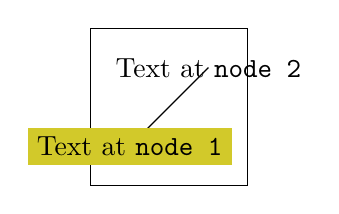
\begin{tikzpicture}
    \draw (0,0) rectangle (2,2);
    \draw (0.5,0.5) node [fill=yellow!80!black]
                           {Text at \verb!node 1!}
         -- (1.5,1.5) node {Text at \verb!node 2!};
\end{tikzpicture}

If the label directly after the \verb+--+ and before the coordinate, 
this places the label in the middle of the line, but the \verb+pos=+ 
options can be used to modify this. Also, options like \verb+near start+ 
and \verb+near end+ can be used to modify this position. You can also 
position labels on curves and, by adding the \verb+sloped+ option, 
have them rotated such that they match the line’s slope. 
Here is an example:\\
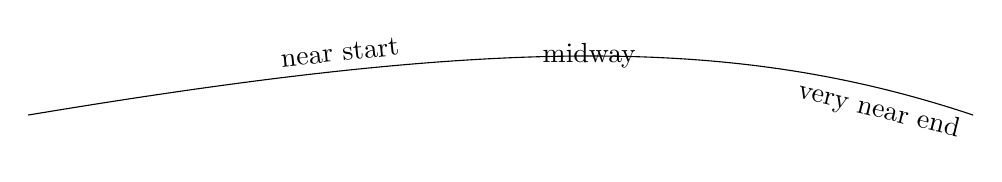
\begin{tikzpicture}
    \draw (0,0) .. controls (6,1) and (9,1) ..
      node[near start,sloped,above] {near start}
      node {midway}
      node[very near end,sloped,below] {very near end} (12,0);
\end{tikzpicture}

%--------------------------------------
\subsection{Diagrams with nodes}

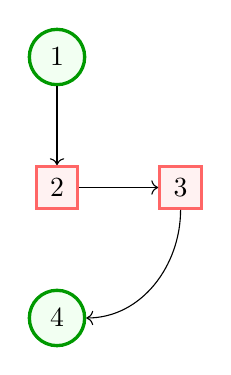
\begin{tikzpicture}[
    roundnode/.style   = {circle, draw=green!60!black, fill=green!5, very thick, 
                          minimum size=20pt},
    squarednode/.style = {rectangle, draw=red!60, fill=red!5, very thick, 
                          minimum size=15pt},
]
    %Nodes
    \node[squarednode]      (maintopic)                              {2};
    \node[roundnode]        (uppercircle)       [above=of maintopic] {1};
    \node[squarednode]      (rightsquare)       [right=of maintopic] {3};
    \node[roundnode]        (lowercircle)       [below=of maintopic] {4};
     
    %Lines
    \draw[->] (uppercircle.south) -- (maintopic.north);
    \draw[->] (maintopic.east) -- (rightsquare.west);
    \draw[->] (rightsquare.south) .. 
              controls +(down:20pt) and +(right:20pt) 
              .. (lowercircle.east);
\end{tikzpicture}

\subsubsection{Extracting Insights From Data diagram}
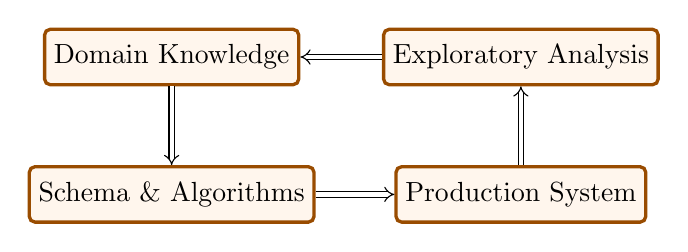
\begin{tikzpicture}[
    squarednode/.style = {rectangle, draw=orange!60!black, fill=orange!7, 
                          very thick, 
                          minimum size=20pt,
                          rounded corners=2pt},
    impliesarrow/.style = {double equal sign distance, -Implies}
]
  
    \node[squarednode] (DK) {Domain Knowledge};
    \node[squarednode] (SA) [below=of DK] {Schema \& Algorithms};
    \node[squarednode] (SP) [right=of SA] {Production System}; 
    \node[squarednode] (EA) [above=of SP] {Exploratory Analysis};

    \draw[impliesarrow] (DK.south) -- (SA.north);
    \draw[impliesarrow] (SA.east) -- (SP.west);
    \draw[impliesarrow] (SP.north) -- (EA.south);
    \draw[impliesarrow] (EA.west) -- (DK.east);
    % \draw[impliesarrow] (DA.north) .. controls +(up:30pt) and +(right:40pt) .. (DK.east);

\end{tikzpicture}

%--------------------------------------
\subsection{Specifying Coordinates}
To appreciate the difference between + and ++ consider the following example:\\
\verb|-- ++(1cm,0cm)  -- ++(0cm,1cm)  -- ++(-1cm,0cm) -- cycle|\\
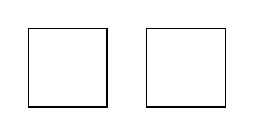
\begin{tikzpicture}
    \def\rectanglepath{-- ++(1cm,0cm)  -- ++(0cm,1cm)  -- ++(-1cm,0cm) -- cycle}
    \draw (0,0) \rectanglepath;
    \draw (1.5,0) \rectanglepath;
\end{tikzpicture}

By comparison, when using a single +, the coordinates are different:\\
\verb|-- +(1cm,0cm)  -- +(1cm,1cm)  -- +(0cm,1cm) -- cycle|\\
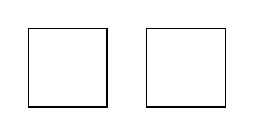
\begin{tikzpicture}
    \def\rectanglepath{-- +(1cm,0cm)  -- +(1cm,1cm)  -- +(0cm,1cm) -- cycle}
    \draw (0,0) \rectanglepath;
    \draw (1.5,0) \rectanglepath;
\end{tikzpicture}

%--------------------------------------
\subsection{Transformations}
\tikz \draw (0,0) -- (0,0.5) [xshift=20pt] (0,0) -- (0,0.5);

\marginpar{
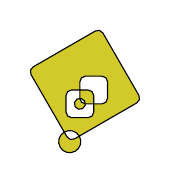
\begin{tikzpicture}[even odd rule,rounded corners=2pt,x=10pt,y=10pt] 
    \filldraw[fill=yellow!80!black]   (0,0) rectangle (1,1) 
                [shift={(0.5,0.5)}]   (0,0) rectangle (1,1)
                        [rotate=30] (-1,-1) rectangle (2,2) 
                                      (0,0) circle (0.2) 
                  [shift={(-1,-1)}]   (0,0) circle (0.4);
\end{tikzpicture}
}

Another way to display all options for arrow tips:\\
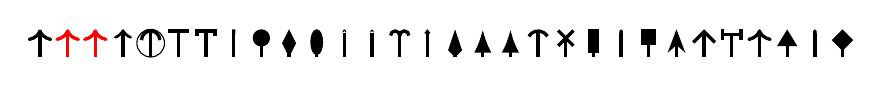
\begin{tikzpicture}
    %  \usetikzlibrary {arrows.meta}
    \def\arrowup{[->,very thick] (0,0) -- (0,10pt)}

    \draw                                   [xshift=-40pt] \arrowup;
    \draw[>=To,red]                         [xshift=-30pt] \arrowup;
    \draw[>=Computer Modern Rightarrow,red] [xshift=-20pt] \arrowup;
    \draw[>=Classical TikZ Rightarrow]      [xshift=-10pt] \arrowup;
    \draw (0,5pt) circle (5pt); % circle to mark Arc Barb
    \draw[>=Arc Barb]                    \arrowup;
    \draw[>=Bar]           [xshift=10pt] \arrowup;
    \draw[>=Bracket]       [xshift=20pt] \arrowup;
    \draw[>=Butt Cap]      [xshift=30pt] \arrowup;
    \draw[>=Circle]        [xshift=40pt] \arrowup;
    \draw[>=Diamond]       [xshift=50pt] \arrowup;
    \draw[>=Ellipse]       [xshift=60pt] \arrowup;
    \draw[>=Fast Round]    [xshift=70pt] \arrowup;
    \draw[>=Fast Triangle] [xshift=80pt] \arrowup;
    \draw[>=Hooks]         [xshift=90pt] \arrowup;
    \draw[>=Implies]       [xshift=100pt] \arrowup;
    \draw[>=Kite]          [xshift=110pt] \arrowup;
    \draw[>=LaTeX]         [xshift=120pt] \arrowup;
    \draw[>=Latex]         [xshift=130pt] \arrowup;
    \draw[>=Parenthesis]   [xshift=140pt] \arrowup;
    \draw[>=Rays]          [xshift=150pt] \arrowup;
    \draw[>=Rectangle]     [xshift=160pt] \arrowup;
    \draw[>=Round Cap]     [xshift=170pt] \arrowup;
    \draw[>=Square]        [xshift=180pt] \arrowup;
    \draw[>=Stealth]       [xshift=190pt] \arrowup;
    \draw[>=Straight Barb] [xshift=200pt] \arrowup;
    \draw[>=Tee Barb]      [xshift=210pt] \arrowup;
    \draw[>=To]            [xshift=220pt] \arrowup;
    \draw[>=Triangle]      [xshift=230pt] \arrowup;
    \draw[>=Triangle Cap]  [xshift=240pt] \arrowup;
    \draw[>=Turned Square] [xshift=250pt] \arrowup;
\end{tikzpicture}

\newpage
%--------------------------------------
\subsection{Repeating Things: For-Loops}

\foreach \i/\t in {
    1/Arc Barb, 2/Bar, 3/Bracket, 4/Butt Cap, 5/Circle, 
    6/Diamond, 7/Ellipse, 8/Fast Round, 9/Fast Triangle, 
    10/Hooks, 11/Implies, 12/Kite, 13/LaTeX, 14/Latex, 
    15/Parenthesis, 16/Rays, 17/Rectangle, 18/Round Cap, 
    19/Square, 20/Stealth, 21/Straight Barb, 22/Tee Barb, 
    23/To, 24/Triangle, 25/Triangle Cap, 26/Turned Square} 
    {\i. \tikz [>=\t] \draw[->,ultra thick] (0,0) -- (15pt,0); \t \\}

\foreach \x in {1,2,3} {$x =\x$, }

\tikz  \foreach \x in {-1,-0.5,...,1} \draw[shift={(\x,0)}] (0,-5pt) -- (0,5pt);

\tikz \foreach \x in {1,...,10} \draw (\x,0) circle (0.4);

\subsubsection{2D tables}
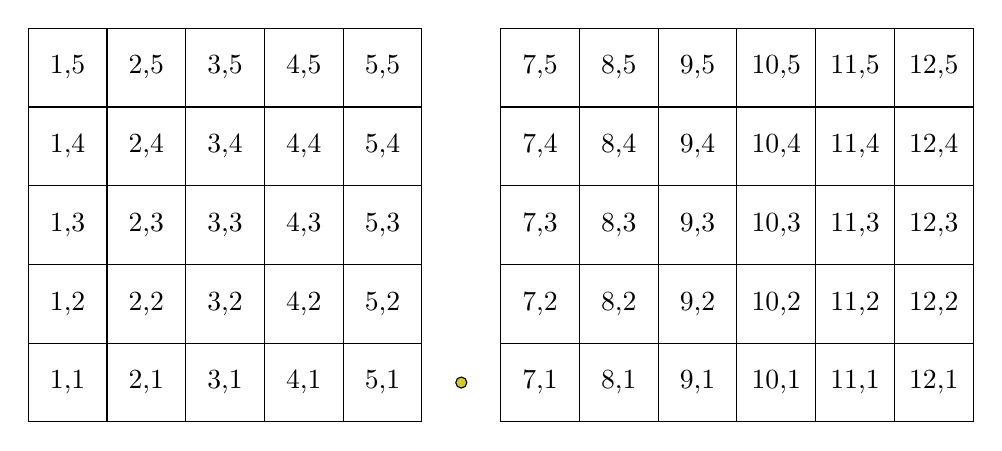
\begin{tikzpicture}
    \filldraw[fill=yellow!80!black] (6,1) circle (2pt);
    \foreach \x in {1,2,...,5,7,8,...,12}
        \foreach \y in {1,...,5}
        {
            \draw (\x,\y) +(-.5,-.5) rectangle ++(.5,.5);
            \draw (\x,\y) node{\x,\y};
        }
\end{tikzpicture}

%--------------------------------------
\subsection{Karl's picture}
\marginpar{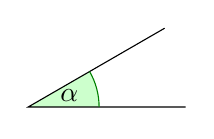
\begin{tikzpicture}
    \coordinate (A) at (2,0);
    \coordinate (B) at (0,0);
    \coordinate (C) at (30:2);
    \draw (A) -- (B) -- (C)
        pic [draw=green!50!black, fill=green!20, angle radius=9mm, "$\alpha$"] 
            {angle = A--B--C};
\end{tikzpicture}}

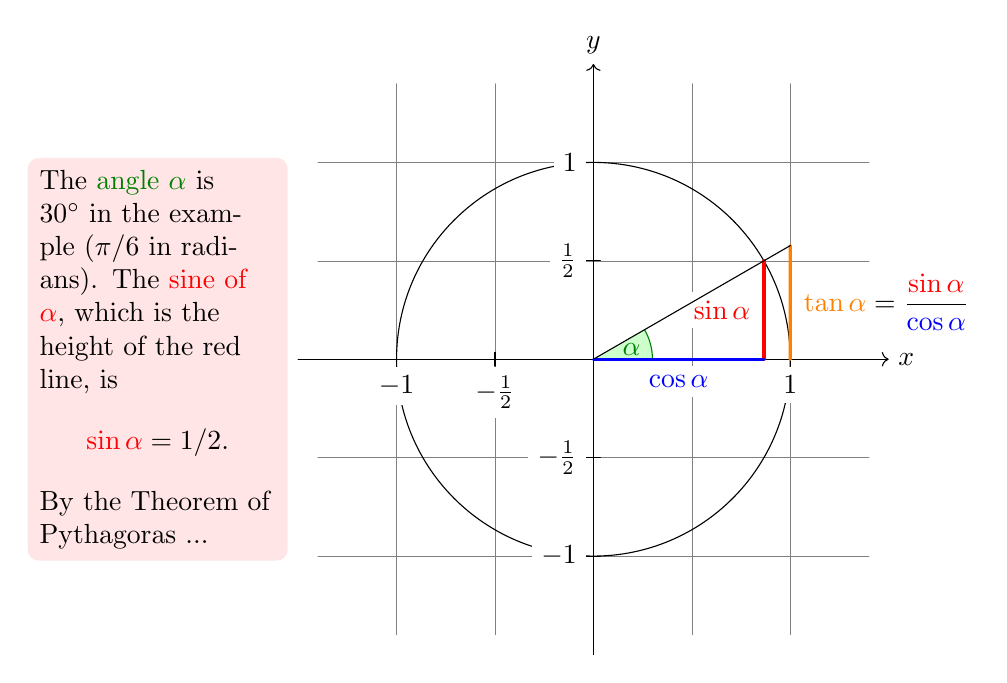
\begin{tikzpicture}
    [scale=2.5,line cap=round,
    % Styles
    axes/.style=,
    grid lines/.style={gray,very thin},
    important line/.style={very thick},
    information text/.style={rounded corners,fill=red!10,inner sep=1ex}]

    % Colors
    \colorlet{anglecolor}{green!50!black}
    \colorlet{sincolor}{red}
    \colorlet{tancolor}{orange!80!black}
    \colorlet{coscolor}{blue}

    % The graphic
    \draw[grid lines,step=.5] (-1.4,-1.4) grid (1.4,1.4);
    \draw (0,0) circle [radius=1cm];

    \begin{scope}[axes]
        \draw[->] (-1.5,0) -- (1.5,0) node[right] {$x$} coordinate(x axis);
        \draw[->] (0,-1.5) -- (0,1.5) node[above] {$y$} coordinate(y axis);

        \foreach \x/\xtext in {-1, -.5/-\frac{1}{2}, 1}
            \draw[xshift=\x cm] (0pt,1pt) -- (0pt,-1pt) node[below,fill=white] {$\xtext$};
        \foreach \y/\ytext in {-1, -.5/-\frac{1}{2}, .5/\frac{1}{2}, 1}
            \draw[yshift=\y cm] (1pt,0pt) -- (-1pt,0pt) node[left,fill=white] {$\ytext$};
    \end{scope}

    \filldraw[fill=green!20,draw=anglecolor] 
        (0,0) -- (3mm,0pt) arc [start angle=0, end angle=30, radius=3mm];
    \draw (15:2mm) node[anglecolor] {$\alpha$};
    
    \draw[important line,sincolor]
        (30:1cm) -- node[left=1pt,fill=white] {$\sin \alpha$} (30:1cm |- x axis); 

    \draw[important line,coscolor]
    (30:1cm |- x axis) -- node[below=2pt,fill=white] {$\cos \alpha$} (0,0);

    % to find tan(30) "geometrically", as an intersection of two lines:
    \path [name path=upward line] (1,0) -- (1,1);
    \path [name path=sloped line] (0,0) -- (30:1.5cm);
    \draw [name intersections={of=upward line and sloped line, by=t}]
          [very thick,orange] (1,0) -- node [right=1pt,fill=white] 
          {$\displaystyle \tan \alpha \color{black}=
          \frac{{\color{red}\sin \alpha}}{\color{blue}\cos \alpha}$} (t);
    \draw (0,0) -- (t);
    
    % text area to the left:
    \draw[xshift=-1.55cm] 
        node[left,text width=3cm,information text] {
            The {\color{anglecolor} angle $\alpha$} is $30^\circ$ in the
            example ($\pi/6$ in radians). 
            The {\color{sincolor}sine of
            $\alpha$}, which is the height of the red line, is
            \[ {\color{sincolor} \sin \alpha} = 1/2. \]
            By the Theorem of Pythagoras ...
        };
\end{tikzpicture}


\newpage
%==============================================================================
\section{Nodes}

\begin{tikzpicture}
    \fill (0,0) circle (1pt);
    \path ( 0,2) node [shape=circle,draw] {}
          ( 0,1) node [shape=circle,draw] {}
          ( 0,0) node [shape=circle,draw] {}
          ( 1,1) node [shape=rectangle,draw] {}
          (-1,1) node [shape=rectangle,draw] {};
  \end{tikzpicture}

%--------------------------------------
\subsection{Placing Nodes Using the At Syntax}

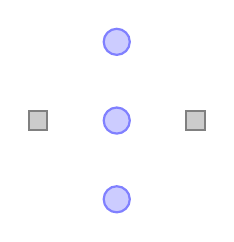
\begin{tikzpicture} [
    place/.style      = {circle,draw=blue!50,fill=blue!20,thick},
    transition/.style = {rectangle,draw=black!50,fill=black!20,thick}
] 
    \node at ( 0,2) [place] {};
    \node at ( 0,1) [place] {};
    \node at ( 0,0) [place] {};
    \node at ( 1,1) [transition] {};
    \node at (-1,1) [transition] {};
\end{tikzpicture}

%--------------------------------------
\subsection{Node size, name and style}

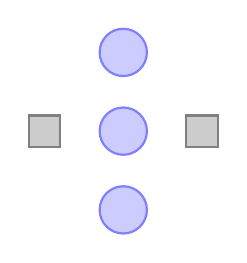
\begin{tikzpicture} [inner sep=2mm,
    place/.style={circle,draw=blue!50,fill=blue!20,thick,
                  inner sep=0pt,minimum size=6mm},
    transition/.style={rectangle,draw=black!50,fill=black!20,thick,
                  inner sep=0pt,minimum size=4mm}
] 
    \node[place]      (waiting 1)      at ( 0,2) {};
    \node[place]      (critical 1)     at ( 0,1) {};
    \node[place]      (semaphore)      at ( 0,0) {};
    \node[transition] (leave critical) at ( 1,1) {};
    \node[transition] (enter critical) at (-1,1) {};
\end{tikzpicture}

%--------------------------------------
\subsection{Labels and pins}

\tikz [
    every label/.style={draw,red,label distance=5mm},
    pin distance=1.5cm
] \node [
    circle,draw,
    pin = right:X,
    pin = above:Y,
    pin = below left:Z,
    label = center:*,
    label = 60:$60^\circ$,
    label = 105:$105^\circ$,
    label = 175:$175^\circ$,
    label = -40:$-40^\circ$,
    label = -95:$-95^\circ$,
    label = -170:$-170^\circ$
] {my circle};


%--------------------------------------
\subsection{Node with tabular text}

\tikz \node [draw] {
    \begin{tabular}{cc}
        upper left & upper right\\
        lower left & lower right
    \end{tabular}
};

%--------------------------------------
\subsection{Gallery}

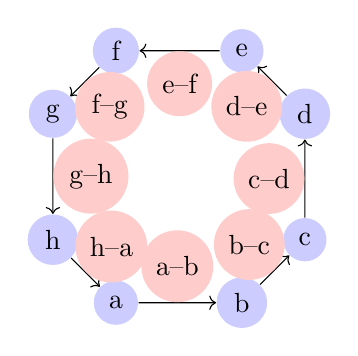
\begin{tikzpicture}
    [scale=.8,auto=left,every node/.style={circle,fill=blue!20}] 
    \node (a) at (-1,-2) {a};
    \node (b) at ( 1,-2) {b};
    \node (c) at ( 2,-1) {c};
    \node (d) at ( 2, 1) {d};
    \node (e) at ( 1, 2) {e};
    \node (f) at (-1, 2) {f};
    \node (g) at (-2, 1) {g};
    \node (h) at (-2,-1) {h};
    
    \foreach \from/\to in {a/b,b/c,c/d,d/e,e/f,f/g,g/h,h/a}
        \draw [->] (\from) -- (\to) node[midway,fill=red!20] {\from--\to}; 
\end{tikzpicture}

\vspace{20pt}

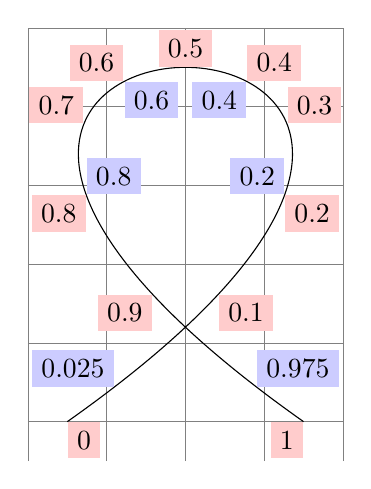
\begin{tikzpicture}[auto]
    \draw[help lines,use as bounding box] (0,-.5) grid (4,5);
    \draw (0.5,0) .. controls (9,6) and (-5,6) .. (3.5,0)
        node foreach \pos in {0,0.1,0.2,0.3,0.4,0.5,0.6,0.7,0.8,0.9,1}
            [pos=\pos,swap,fill=red!20] {\pos}
        node foreach \pos in {0.025,0.2,0.4,0.6,0.8,0.975}
            [pos=\pos,fill=blue!20] {\pos}; 
\end{tikzpicture}

\vspace{20pt}

% \usetikzlibrary {automata}
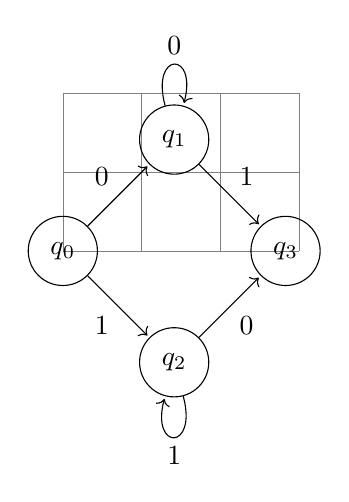
\begin{tikzpicture}[shorten >=1pt,node distance=2cm,auto]
    \draw[help lines] (0,0) grid (3,2);
  
    \node[state] (q_0) {$q_0$}; 
    \node[state] (q_1) [above right of=q_0] {$q_1$}; 
    \node[state] (q_2) [below right of=q_0] {$q_2$}; 
    \node[state] (q_3) [below right of=q_1] {$q_3$};
    
    \path[->] (q_0) edge              node        {0} (q_1)
                    edge              node [swap] {1} (q_2)
              (q_1) edge              node        {1} (q_3)
                    edge [loop above] node        {0} ()
              (q_2) edge              node [swap] {0} (q_3)
                    edge [loop below] node        {1} ();
\end{tikzpicture}

\end{document}